\documentclass[11pt,a4paper]{article}

\usepackage[margin=2.3cm]{geometry}
\usepackage[T1]{fontenc}
\usepackage{lmodern}
\usepackage{amsmath}
\usepackage{booktabs}
\usepackage{caption}
\usepackage{float}
\usepackage{graphicx}
\usepackage{pgfplots}
\pgfplotsset{compat=1.17}
\usetikzlibrary{arrows.meta}
\usepackage[hidelinks]{hyperref}

\definecolor{blue1}{HTML}{1F77B4}
\definecolor{red1}{HTML}{D62728}
\definecolor{green1}{HTML}{2CA02C}

\setlength{\parskip}{0.5em}
\setlength{\parindent}{0pt}

\newcommand{\good}[1]{\textcolor{green1}{#1}}
\newcommand{\bad}[1]{\textcolor{red1}{#1}}
\newcommand{\cnend}{\textit{cn-end}}

\title{GigaSketch: Sketch-to-Image with Stable Diffusion 1.5 and ControlNet}
\author{Ngoc Minh Le}
\date{\today}

\begin{document}
\maketitle

% ---------------------------------------------------------------------------
\section*{Introduction}

For this project I built GigaSketch, a small tool that turns rough stick-figure sketches into realistic
``Gigachad'' images while keeping the pose of the drawing. It runs on a pretrained Stable Diffusion 1.5
\cite{rombach2022} with a Scribble ControlNet \cite{zhang2023}, with no training involved.

I went with a meme theme: six sketches become dramatic black-and-white ``gigachad-style'' photos of very
muscular guys. The style only comes from the text prompt; I don't copy any real person's face.

What I ended up with:
\begin{itemize}
  \item a preprocessing step that cleans a photo or scan of a sketch into a scribble map;
  \item a prompt template, so I only describe what is in the sketch and the style is added for me;
  \item an analysis of \texttt{control\_guidance\_end} (I call it \cnend), the setting that decides between
        keeping the pose and getting natural faces;
  \item a command-line tool and a Gradio web UI.
\end{itemize}

Code: \url{https://github.com/hocgiacontrung/gigasketch}

% ---------------------------------------------------------------------------
\section*{Method}

The basic idea: the sketch decides \emph{where} things go, and the text prompt decides \emph{what} they turn
into. Figure~\ref{fig:pipeline} shows how the pieces fit together.

\begin{figure}[H]
\centering
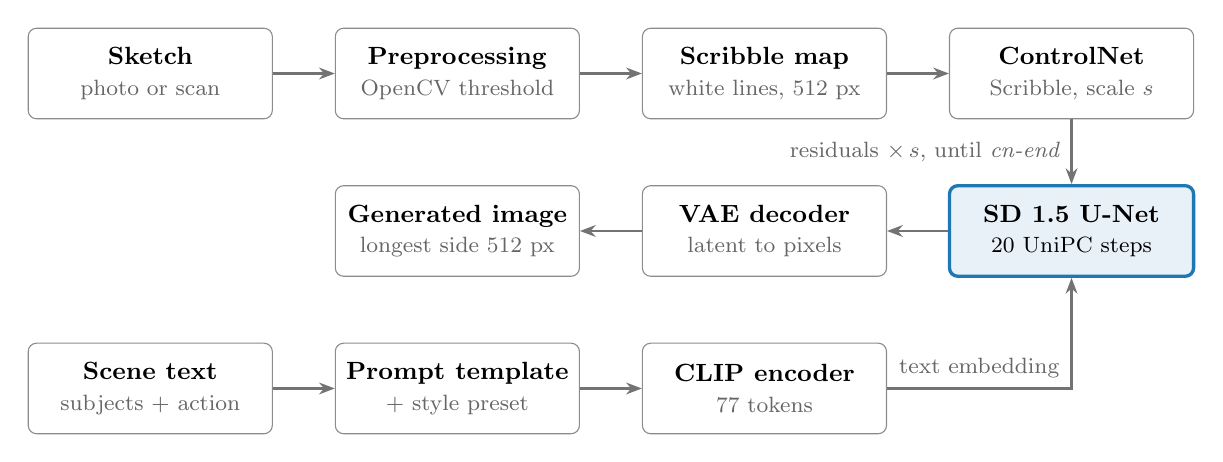
\begin{tikzpicture}[
    box/.style={draw=black!45, rounded corners=3pt, minimum width=3.1cm, minimum height=1.15cm,
                align=center, font=\small},
    main/.style={box, draw=blue1, fill=blue1!10, very thick},
    arr/.style={-{Stealth[length=2mm]}, black!55, thick},
    note/.style={font=\footnotesize, text=black!60}]
  % sketch path (top row)
  \node[box]  (sketch) at (0,0)     {\textbf{Sketch}\\{\footnotesize\color{black!60}photo or scan}};
  \node[box]  (prep)   at (3.9,0)   {\textbf{Preprocessing}\\{\footnotesize\color{black!60}OpenCV threshold}};
  \node[box]  (map)    at (7.8,0)   {\textbf{Scribble map}\\{\footnotesize\color{black!60}white lines, 512 px}};
  \node[box]  (cnet)   at (11.7,0)  {\textbf{ControlNet}\\{\footnotesize\color{black!60}Scribble, scale $s$}};
  % generation (middle row)
  \node[main] (unet)   at (11.7,-2) {\textbf{SD 1.5 U-Net}\\{\footnotesize 20 UniPC steps}};
  \node[box]  (vae)    at (7.8,-2)  {\textbf{VAE decoder}\\{\footnotesize\color{black!60}latent to pixels}};
  \node[box]  (img)    at (3.9,-2)  {\textbf{Generated image}\\{\footnotesize\color{black!60}longest side 512 px}};
  % text path (bottom row)
  \node[box]  (scene)  at (0,-4)    {\textbf{Scene text}\\{\footnotesize\color{black!60}subjects + action}};
  \node[box]  (tmpl)   at (3.9,-4)  {\textbf{Prompt template}\\{\footnotesize\color{black!60}+ style preset}};
  \node[box]  (clip)   at (7.8,-4)  {\textbf{CLIP encoder}\\{\footnotesize\color{black!60}77 tokens}};
  % arrows
  \draw[arr] (sketch) -- (prep);
  \draw[arr] (prep) -- (map);
  \draw[arr] (map) -- (cnet);
  \draw[arr] (cnet) -- node[note, left] {residuals $\times\, s$, until \cnend} (unet);
  \draw[arr] (unet) -- (vae);
  \draw[arr] (vae) -- (img);
  \draw[arr] (scene) -- (tmpl);
  \draw[arr] (tmpl) -- (clip);
  \draw[arr] (clip.east) -| node[note, above, pos=0.25] {text embedding} (unet.south);
\end{tikzpicture}
\caption{The GigaSketch pipeline. Only the scribble map goes through ControlNet; the text reaches the U-Net
through CLIP. \cnend{} decides for how many of the 20 steps ControlNet gets to push.}
\label{fig:pipeline}
\end{figure}

\textbf{Preprocessing (OpenCV).} First the sketch is resized so its longest side is 512 px (SD needs
multiples of 8). A light blur removes the paper texture, then an adaptive threshold (block 51, $C = 15$) turns
the lines white on a black background, which is what the Scribble ControlNet was trained on. Started with a
block size of 15, but it turned thick strokes into double outlines, so I went up to 51. Finally a small opening
removes specks and a dilation makes the strokes a bit thicker.

\textbf{ControlNet Scribble.} ControlNet is basically a trainable copy of the SD U-Net encoder, connected
through zero-initialised convolutions. It looks at the scribble map and adds its features to the U-Net's skip
connections at every denoising step, multiplied by the conditioning scale $s$. The original SD 1.5 weights
stay frozen.

\textbf{Stable Diffusion 1.5.} SD works on a $64\times64$ latent (the VAE shrinks 512 px by 8) and denoises it
in 20 UniPC steps \cite{zhao2023}, with classifier-free guidance \cite{ho2022} $w = 7.5$ and a CLIP text encoder
\cite{radford2021} that reads up to 77 tokens. With the ControlNet residuals $C(x)$ from the scribble map $x$,
each step predicts:
\begin{equation}
  \hat\epsilon = \epsilon_\theta\big(z_t, \varnothing, s\,C(x)\big)
     + w\,\Big[\epsilon_\theta\big(z_t, c, s\,C(x)\big) - \epsilon_\theta\big(z_t, \varnothing, s\,C(x)\big)\Big]
\end{equation}

\textbf{Prompt template.} I only want the user to describe the scene: who is there and what they are doing.
The script then builds
\begin{center}
  \small\texttt{"\{content\}, \{style preset\}, highly detailed, sharp focus, best quality"}
\end{center}
plus a negative prompt from a base list and the preset's own terms. The presets are \texttt{gigachad},
\texttt{photo}, \texttt{anime}, \texttt{comic} and \texttt{custom} (no preset, you write the style yourself).

\textbf{\cnend.} \texttt{control\_guidance\_end} is the fraction of the steps where $C(x)$ is applied; after
that, SD continues from the text alone. Since SD decides big shapes early and details late, this one number
ends up trading the pose against freedom in the details (see Experiments). I use 0.4 by default for photo
styles and 1.0 for drawn styles.

% ---------------------------------------------------------------------------
\section*{Implementation and setup}

Everything is built with Hugging Face Diffusers, in two Python files, and runs on my laptop GPU (8 GB).

\begin{table}[H]
\centering
\caption{Models, libraries and hardware.}
\begin{tabular}{lp{11.5cm}}
\toprule
Part & Choice \\
\midrule
Base model & \texttt{stable-diffusion-v1-5/stable-diffusion-v1-5}, fp16, safety checker off \\
Optional base model & Realistic Vision 5.1 + \texttt{sd-vae-ft-mse} VAE (\texttt{-{}-model realistic}) \\
ControlNet & \texttt{lllyasviel/control\_v11p\_sd15\_scribble} \\
Scheduler & UniPC, 20 steps \\
Libraries & PyTorch 2.14 (CUDA 12.6), Diffusers 0.43, Transformers 5.23, OpenCV 5.1, Gradio 6.32 \\
Hardware & NVIDIA RTX 4060 Laptop, 8 GB VRAM; a few seconds per image \\
\bottomrule
\end{tabular}
\end{table}

\texttt{src/generate.py} has the preprocessing, the prompt template, the pipeline and a CLI. With
\texttt{-{}-seeds 42 43 44 45} it loads the model once and saves every image, a sketch\,|\,control
map\,|\,result comparison, and one grid per sketch. The file names contain all the settings (style, scale,
\cnend, guidance, seed), so every figure here can be regenerated, and the README has the exact prompt for each
sketch.

\texttt{src/app.py} is the Gradio web UI (Figure~\ref{fig:ui}). You upload or draw a sketch, describe it, and
pick the style, base model and \cnend{} with a slider. The slider jumps to the style's default when you switch
styles, and the other settings (scale, guidance, steps, seed) are in a collapsed panel.

\begin{figure}[H]
\centering
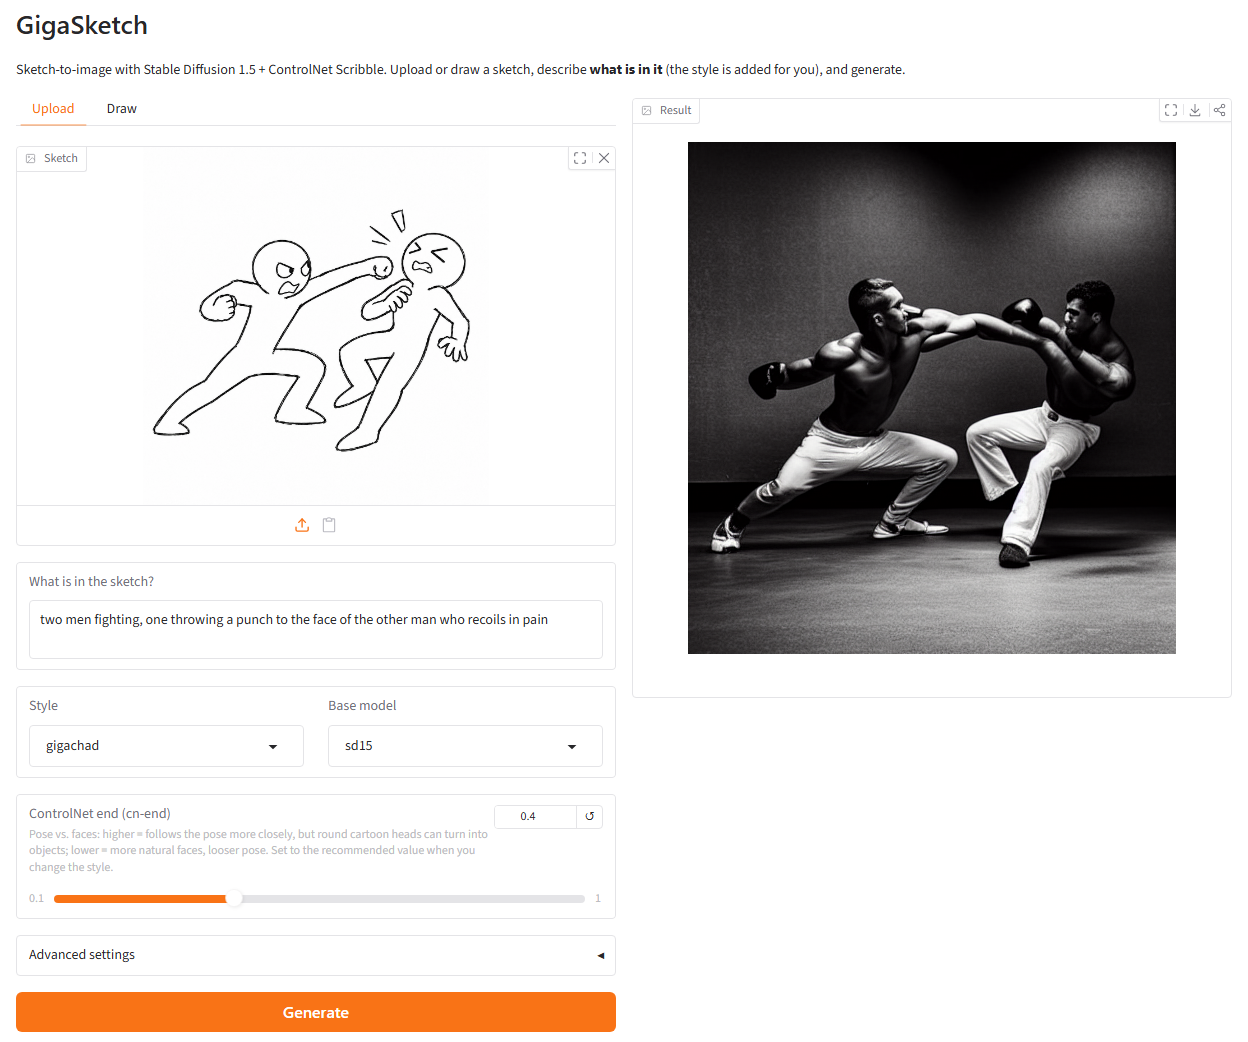
\includegraphics[width=0.82\textwidth]{figures/fig_ui.png}
\caption{The web UI with the m4 sketch: upload or draw on the left, the description, style, base model and
\cnend{} slider below it, and the result on the right.}
\label{fig:ui}
\end{figure}

% ---------------------------------------------------------------------------
\section*{Results}

With the default settings (gigachad style, scale 1.0, \cnend{} 0.4), five out of six sketches keep their pose
in at least 3 of 4 seeds. Figure~\ref{fig:results} shows every sketch with seeds 42 to 45.

\begin{table}[H]
\centering
\caption{Pose preservation over seeds 42--45 with the default settings.}
\begin{tabular}{lp{4.6cm}cp{6.2cm}}
\toprule
Sketch & Scene & Pose kept & Notes \\
\midrule
m1 & one man holding another's cheek & \good{4/4} & very stable; close-up faces \\
m5 & a dunk, a second man with crossed arms & \good{4/4} & dunk, ball and crossed arms in every seed \\
m4 & a punch, the victim recoils & \good{4/4} & seed 42 adds frame artifacts, seed 44 a light beam \\
m6 & four friends posing & \good{4/4} & 3 men + 1 woman as asked; spiky hair becomes hair blobs \\
m3 & one man bored, one laughing & 3/4 & real faces, but the hand on the cheek is lost \\
m2 & a slap (rough pencil sketch) & \bad{0/4} & failure case, see Limitations \\
\bottomrule
\end{tabular}
\end{table}

\textbf{m1} is the most stable: both faces and the hand on the cheek are there every time. \textbf{m5} is my
favourite: the jump, the ball overhead and the crossed arms come through in every seed. \textbf{m4} keeps the
lunge and the punch, and \textbf{m6} keeps all four poses, even the guy crouching in front. \textbf{m3} shows
the downside of \cnend{} 0.4: both guys get real faces, but small details like the hand on the cheek get lost.

\begin{figure}[H]
\centering
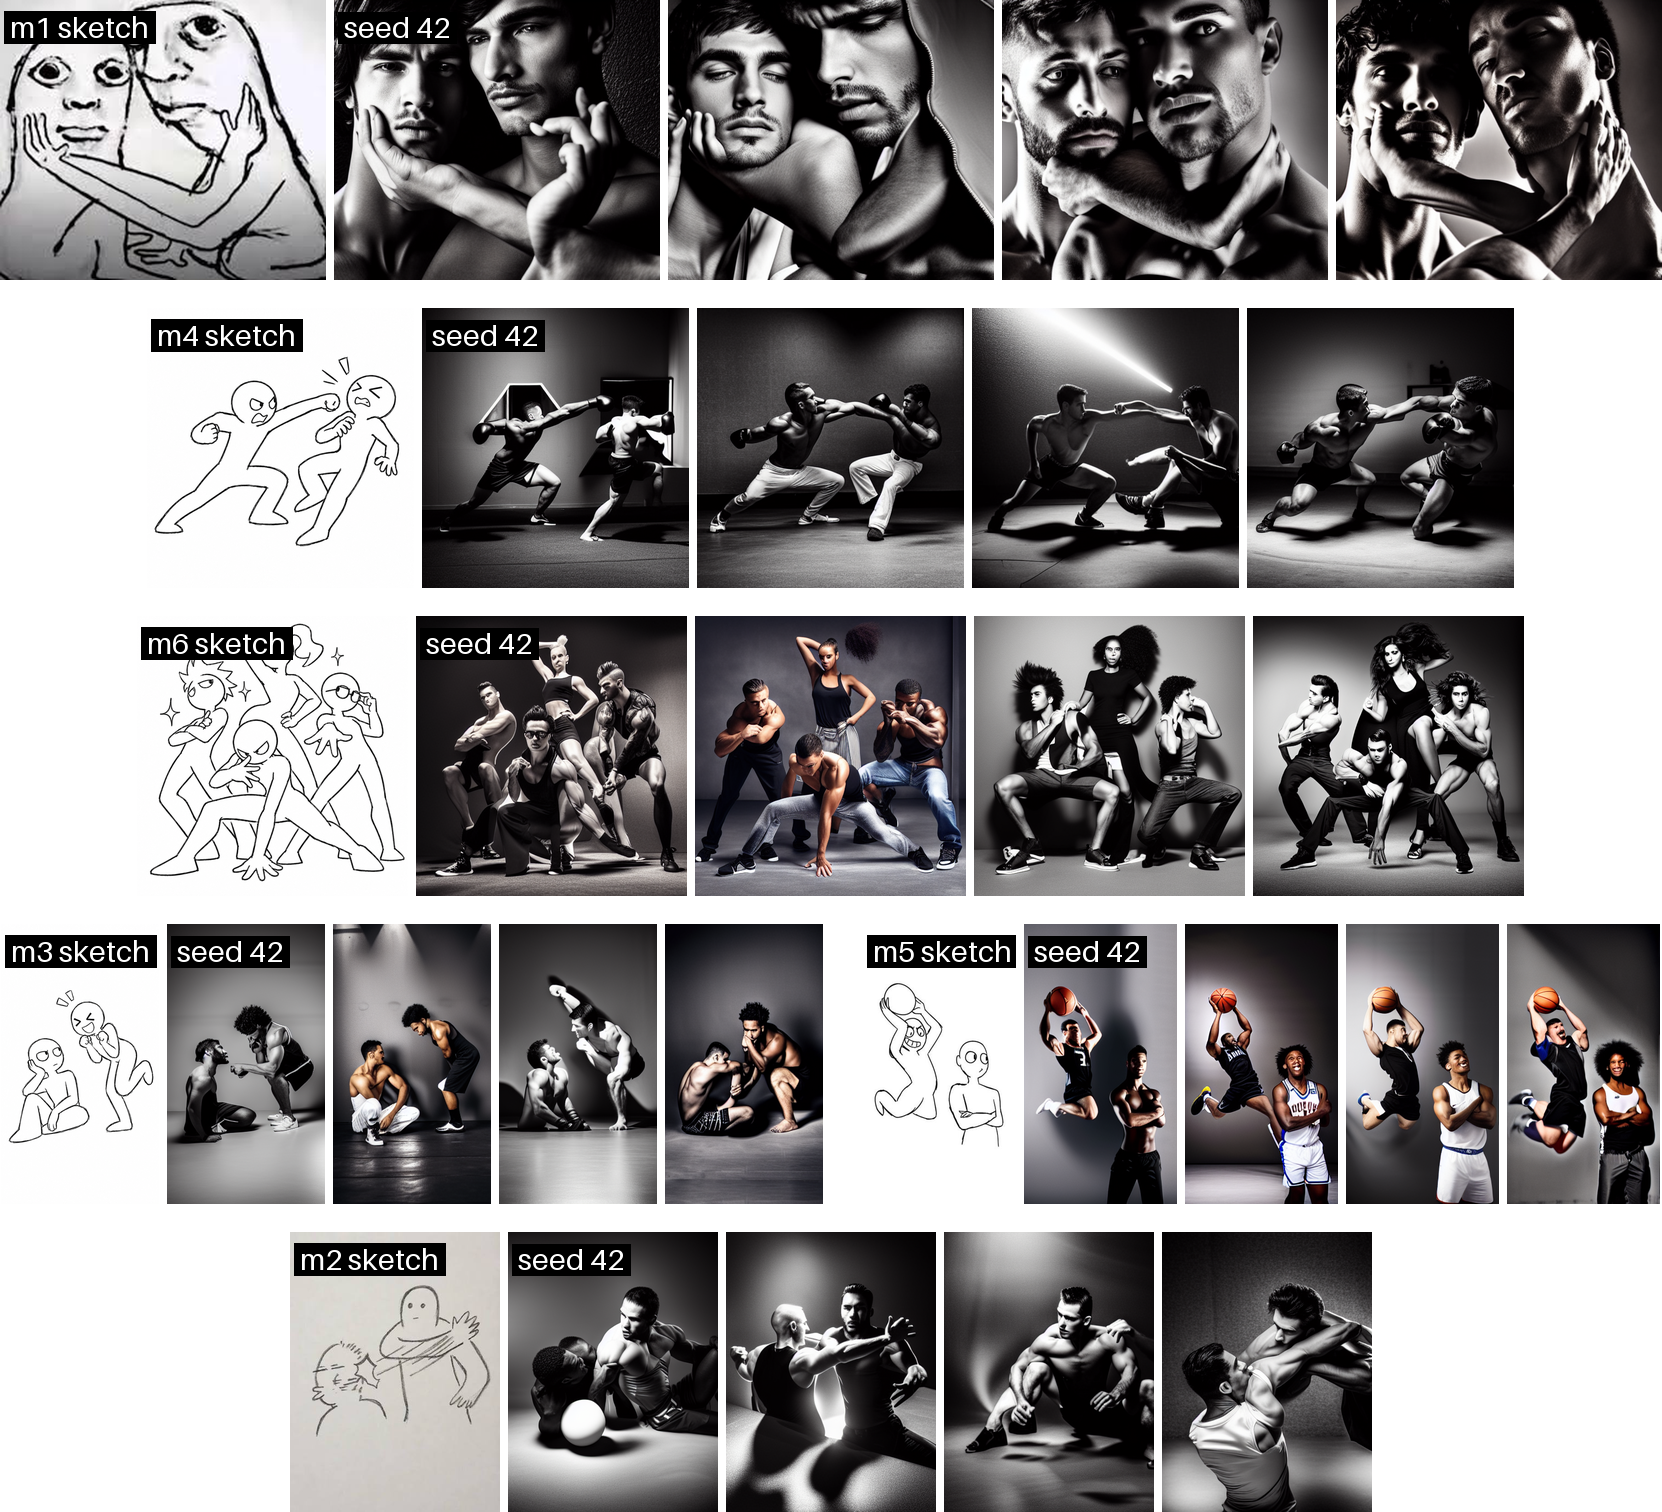
\includegraphics[width=\textwidth]{figures/fig_results.png}
\caption{Each sketch with seeds 42, 43, 44 and 45 (gigachad style, scale 1.0, \cnend{} 0.4). Rows from top:
m1; m4; m6; m3 and m5; m2 (failure case).}
\label{fig:results}
\end{figure}

% ---------------------------------------------------------------------------
\section*{Experiments and analysis}

The biggest thing I learned: \cnend{} is a trade-off between pose and faces, and no single value works for
every sketch. Everything below uses seed 42 unless I say otherwise.

\begin{table}[H]
\centering
\caption{Experiments.}
\begin{tabular}{p{2.6cm}p{4.2cm}p{7.9cm}}
\toprule
Experiment & Compared & What happened \\
\midrule
ControlNet scale & 1.0 vs 1.3 & 1.3 was worse on every sketch: it follows round heads and dot eyes even more
  literally \\
Prompt content & scene only vs scene + action & without the action (``slapping''), m2's motion lines turned
  into objects \\
Negative prompt & + \texttt{helmet, mask, hat, covered face} & did nothing on its own; the heads stayed
  helmets \\
\cnend & 1.0, 0.8, 0.7, 0.6, 0.5, 0.4 & see below \\
Sketch quality & first vs redrawn m3/m4 & my first versions (big heads, grid teeth) became a glass sphere and
  a speaker; clean full-body redraws kept the pose \\
Base model & SD 1.5 vs Realistic Vision 5.1 \cite{realisticvision}, 2 seeds & nicer skin and anatomy on m6,
  face paint on m4, and on m3 one person disappeared in both seeds \\
Drawn styles & anime and comic, \cnend{} 0.4 vs 1.0 & at 0.4 the jumping guy in m5 disappeared; at 1.0 the
  pose is back \\
\bottomrule
\end{tabular}
\end{table}

\textbf{\cnend.} With 20 steps, \cnend{} 0.4 means ControlNet only works during the first 8 steps. Going from
1.0 down to 0.6 barely changes anything, because the layout and the head shapes are already fixed in roughly
the first half. Everything happens between 0.5 and 0.4: above that, the big empty circles of the cartoon heads
turn into helmets, bowls or glass spheres; at 0.4 SD has enough free steps to draw real faces, but the pose
gets looser (Figure~\ref{fig:cnend}).

\begin{figure}[H]
\centering
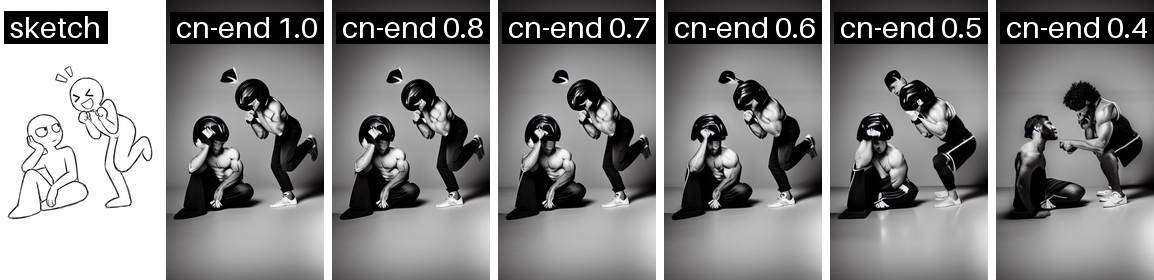
\includegraphics[width=\textwidth]{figures/fig_cnend_m3.png}
\caption{m3, seed 42, \cnend{} from 1.0 to 0.4. The heads stay helmets down to 0.5 and become faces at 0.4,
where the hand on the cheek and the kick are lost.}
\label{fig:cnend}
\end{figure}

The best value also depends on the sketch: m4 looks best at 0.5, m6 only works at 0.4, and m1 and m5 are fine
with anything. It even depends on the seed: at \cnend{} 1.0, only seed 42 (out of 42 to 45) turned m3's heads
into helmets. So instead of one fixed value, I use 0.4 for photo styles, where round heads are the main
problem, and 1.0 for anime and comic, where round heads are just normal. In the UI it is a slider, so you can
pick yourself.

% ---------------------------------------------------------------------------
\section*{Limitations and failure case}

m2, a rough pencil slap, fails in all 4 seeds. The people look real, but you can't tell it is a slap. The
motion lines, the impact star and the hatching all get read as edges of objects, so they turn into balls, hats
or extra limbs. ControlNet can't tell a symbol from an outline: clean outlines work, symbols don't.

\begin{itemize}
  \item \textbf{Sketch vs.\ realism.} ControlNet forces a photo onto cartoon proportions (huge round heads,
        noodle arms). The more closely it follows them, the weirder the result looks.
  \item \textbf{Model size.} SD 1.5 works at 512 px, so a face 40 px wide is only about $5\times5$ latent
        pixels, which is why small faces look smeared. Hands and several people interacting are also known
        weak spots.
  \item \textbf{Text encoder.} CLIP only reads 77 tokens and isn't good with relations between people: in m6,
        ``one woman'' first turned everyone into a woman.
  \item \textbf{Exaggerated features} can still turn into strange details, like spiky hair becoming hair blobs.
\end{itemize}

Bigger models (SDXL, Flux, DALL$\cdot$E~3) are better at anatomy and prompts, but they need more VRAM or are
closed, and the closed ones don't follow a sketch as strictly as ControlNet does.

% ---------------------------------------------------------------------------
\section*{Conclusion}

Overall, a pretrained SD 1.5 with a Scribble ControlNet can turn clean stick-figure sketches into photos that
keep the pose, without any training. Five of my six sketches keep their pose in at least 3 of 4 seeds. The
setting that matters most is \cnend: it trades the pose against natural faces, so I made it a per-style default
and a slider in the UI instead of one fixed number.

If I had more time, I would try, in this order:
\begin{enumerate}
  \item SDXL with an SDXL scribble ControlNet, for 1024 px images and better anatomy.
  \item A LoRA fine-tuned on the gigachad style, so the look doesn't depend on long prompts.
  \item Removing symbols (motion lines, impact stars) from the sketch before ControlNet sees it.
\end{enumerate}

Sketches: m1 and m2 are internet memes; I drew m3 to m6 myself.

% ---------------------------------------------------------------------------
\begin{thebibliography}{9}

\bibitem{rombach2022}
R.~Rombach, A.~Blattmann, D.~Lorenz, P.~Esser and B.~Ommer.
\newblock High-resolution image synthesis with latent diffusion models.
\newblock In \emph{CVPR}, 2022. \url{https://arxiv.org/abs/2112.10752}.
\newblock Weights: \url{https://huggingface.co/stable-diffusion-v1-5/stable-diffusion-v1-5}.

\bibitem{zhang2023}
L.~Zhang, A.~Rao and M.~Agrawala.
\newblock Adding conditional control to text-to-image diffusion models.
\newblock In \emph{ICCV}, 2023. \url{https://arxiv.org/abs/2302.05543}.
\newblock Weights: \url{https://huggingface.co/lllyasviel/control_v11p_sd15_scribble}.

\bibitem{zhao2023}
W.~Zhao, L.~Bai, Y.~Rao, J.~Zhou and J.~Lu.
\newblock UniPC: A unified predictor-corrector framework for fast sampling of diffusion models.
\newblock In \emph{NeurIPS}, 2023. \url{https://arxiv.org/abs/2302.04867}.

\bibitem{ho2022}
J.~Ho and T.~Salimans.
\newblock Classifier-free diffusion guidance.
\newblock 2022. \url{https://arxiv.org/abs/2207.12598}.

\bibitem{radford2021}
A.~Radford et al.
\newblock Learning transferable visual models from natural language supervision.
\newblock In \emph{ICML}, 2021. \url{https://arxiv.org/abs/2103.00020}.

\bibitem{realisticvision}
SG161222.
\newblock Realistic Vision 5.1 (CreativeML OpenRAIL-M), with the VAE \texttt{stabilityai/sd-vae-ft-mse}.
\newblock \url{https://huggingface.co/SG161222/Realistic_Vision_V5.1_noVAE}.

\bibitem{libs}
Libraries: Diffusers (\url{https://github.com/huggingface/diffusers}),
Transformers (\url{https://github.com/huggingface/transformers}), PyTorch (\url{https://pytorch.org}),
OpenCV (\url{https://opencv.org}), Gradio (\url{https://www.gradio.app}).

\end{thebibliography}

\end{document}
